%% LyX 2.3.7 created this file.  For more info, see http://www.lyx.org/.
%% Do not edit unless you really know what you are doing.
\documentclass[10pt,english,t,10pt]{beamer}
\usepackage{lmodern}
\usepackage[T1]{fontenc}
\usepackage[utf8]{inputenc}
\setcounter{tocdepth}{1}
\setlength{\parskip}{\smallskipamount}
\setlength{\parindent}{0pt}
\usepackage{babel}
\usepackage{amsbsy}
\usepackage{amstext}
\usepackage{amssymb}
\usepackage{graphicx}
\usepackage[authoryear]{natbib}
\PassOptionsToPackage{normalem}{ulem}
\usepackage{ulem}
\ifx\hypersetup\undefined
  \AtBeginDocument{%
    \hypersetup{unicode=true}
  }
\else
  \hypersetup{unicode=true}
\fi

\makeatletter
%%%%%%%%%%%%%%%%%%%%%%%%%%%%%% Textclass specific LaTeX commands.
% this default might be overridden by plain title style
\newcommand\makebeamertitle{\frame{\maketitle}}%
% (ERT) argument for the TOC
\AtBeginDocument{%
  \let\origtableofcontents=\tableofcontents
  \def\tableofcontents{\@ifnextchar[{\origtableofcontents}{\gobbletableofcontents}}
  \def\gobbletableofcontents#1{\origtableofcontents}
}

%%%%%%%%%%%%%%%%%%%%%%%%%%%%%% User specified LaTeX commands.



\usepackage{tikz}
\usetikzlibrary{positioning}
\usepackage{appendixnumberbeamer}

\usepackage{graphicx}
\usepackage{subfig}

\usetheme[progressbar=frametitle,block=fill,subsectionpage=progressbar]{metropolis}

% margin
\setbeamersize{text margin right=1.5cm}

% colors
\definecolor{DarkRed}{rgb}{0.7,0,0}
%\colorlet{DarkRed}{red!70!black}
\setbeamercolor{normal text}{fg=black}
\setbeamercolor{alerted text}{fg=DarkRed}
\setbeamercolor{progress bar}{fg=DarkRed}
\setbeamercolor{button}{bg=DarkRed}

% width of seperators
\makeatletter
\setlength{\metropolis@titleseparator@linewidth}{1pt}
\setlength{\metropolis@progressonsectionpage@linewidth}{1pt}
\setlength{\metropolis@progressinheadfoot@linewidth}{1pt}
\makeatother

% new alert block
\newlength\origleftmargini
\setlength\origleftmargini\leftmargini
\setbeamertemplate{itemize/enumerate body begin}{\setlength{\leftmargini}{4mm}}
\let\oldalertblock\alertblock
\let\oldendalertblock\endalertblock
\def\alertblock{\begingroup \setbeamertemplate{itemize/enumerate body begin}{\setlength{\leftmargini}{\origleftmargini}} \oldalertblock}
\def\endalertblock{\oldendalertblock \endgroup}
\setbeamertemplate{mini frame}{}
\setbeamertemplate{mini frame in current section}{}
\setbeamertemplate{mini frame in current subsection}{}
\setbeamercolor{section in head/foot}{fg=normal text.bg, bg=structure.fg}
\setbeamercolor{subsection in head/foot}{fg=normal text.bg, bg=structure.fg}

% footer
\makeatletter
\setbeamertemplate{footline}{%
    \begin{beamercolorbox}[colsep=1.5pt]{upper separation line head}
    \end{beamercolorbox}
    \begin{beamercolorbox}{section in head/foot}
      \vskip1pt\insertsectionnavigationhorizontal{\paperwidth}{}{\hskip0pt plus1filll \insertframenumber{} / \inserttotalframenumber \hskip2pt}\vskip3pt% 
    \end{beamercolorbox}%
    \begin{beamercolorbox}[colsep=1.5pt]{lower separation line head}
    \end{beamercolorbox}
}
\makeatother

% toc
\setbeamertemplate{section in toc}{\hspace*{1em}\inserttocsectionnumber.~\inserttocsection\par}
\setbeamertemplate{subsection in toc}{\hspace*{2em}\inserttocsectionnumber.\inserttocsubsectionnumber.~\inserttocsubsection\par}

\usepackage{comment} 

\makeatother

\begin{document}
\title{1. Introduction\vspace{-2mm}}
\subtitle{Adv. Macro: Heterogenous Agent Models} 
\author{Nicolai Waldstrøm}
\date{2024}

{
\setbeamertemplate{footline}{} 
\begin{frame}

\maketitle

\begin{tikzpicture}[overlay, remember picture]
\node[above left=0cm and 0.0cm of current page.south east] 
{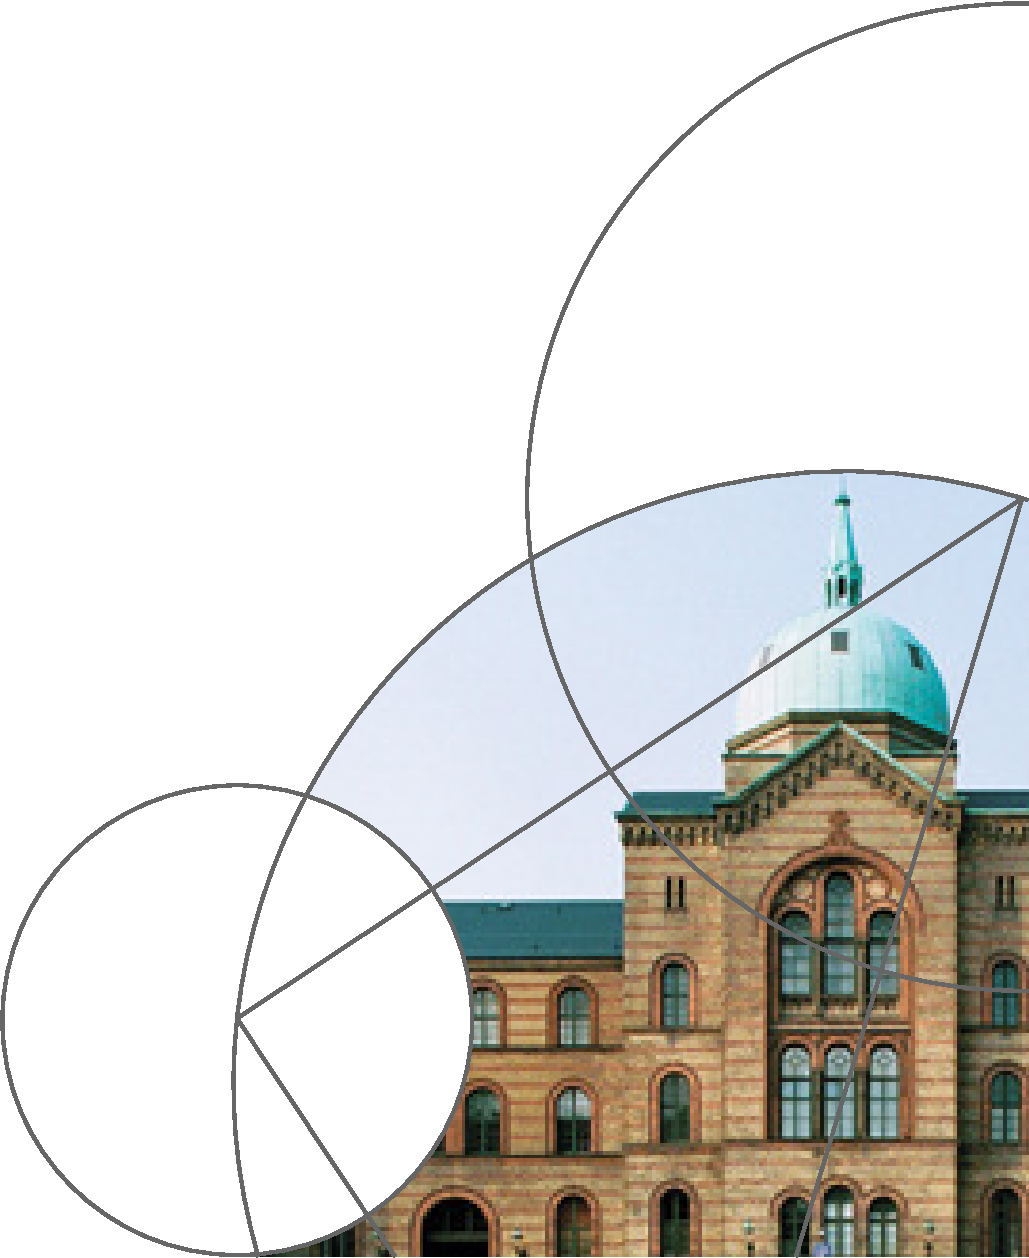
\includegraphics[width=4cm]{figs/KUSAMFtitlelrcorner.pdf}};
\end{tikzpicture}

\begin{tikzpicture}[overlay, remember picture]
\node[below left=0.5cm and .8cm of current page.north east] 
{\includegraphics[width=1.5cm]{figs/KUSAMFlogo.pdf}};
\end{tikzpicture}


\end{frame}
}

\addtocounter{framenumber}{-1}

\section{Introduction}
\begin{frame}{Introduction}
\vspace{-2mm}
\begin{itemize}
\item <+->\textbf{Teacher: }Nicolai Waldstrøm
\item <+->\textbf{Central economic questions:}
\begin{enumerate}
\item What explains the level and dynamics of heterogeneity/inequality?
\item What role does heterogeneity play for understanding consumption-saving
dynamics in partial equilibrium?
\item What role does heterogeneity play for understanding business-cycle
fluctuations in general equilibrium?
\end{enumerate}
\item <+->\textbf{Central technical method:} Programming in Python

\textbf{Prerequisite:} \emph{Intro. to Programming and Numerical Analysis}

\textbf{Complicated:} \emph{Close to the research frontier}
\item <+->\textbf{Plan for today:}
\begin{enumerate}
\item More about the course
\item Consumption-saving models
\item Numerical dynamic programming
\end{enumerate}
\end{itemize}
\end{frame}
%
\begin{frame}{Macroeconomic Models with Heterogeneous Agents}
\begin{itemize}
\item <+->\vspace{-2mm}\textbf{Model components:}
\begin{enumerate}
\item Optimizing individual agents (households + firms)
\item Idiosyncratic and aggregate risk (\emph{uncertainty})
\item Information flows (who knows what when $\Rightarrow$ often everything)
\item Market clearing
\end{enumerate}
\item <+->\textbf{Insurance/markets:}

\emph{Complete} $\rightarrow$ idiosyncratic risk insured away $\sim$
representative agent

\emph{Incomplete} $\rightarrow$ agents need to \emph{self-insure
}by saving
\item <+->\textbf{Heterogeneity:}

\emph{Ex ante }in\emph{ }preferences, abilities etc.

\emph{Ex post} after realization of idiosyncratic shocks
\item <+->\textbf{HANC: }Heterogeneous Agent \emph{Neo-Classical }model\\
{\footnotesize{}(Aiyagari-Bewley-Hugget-Imrohoroglu or Standard Incomplete
Market model)}{\footnotesize\par}
\item <+->\textbf{HANK: }Heterogeneous Agent \emph{New Keynesian} model\\
(i.e. include price and wage setting frictions)
\end{itemize}
\end{frame}
%
\begin{frame}{Teaching method}
\begin{itemize}
\item <+->\textbf{Lectures: }Wednesday 15-18

\textasciitilde 2 hours of >>normal<< lecture

\textasciitilde 1 hour of active problem solving (no exercise classes)
\item <+->\textbf{Content:}
\begin{enumerate}
\item Explanation of computational methods
\item Discussion of research papers
\item Examples of code for central mechanisms

(you should run the notebook codes simultaneously)
\end{enumerate}
\item <+->\textbf{Material:}\vspace{1mm}

{\small{}Web: }\textcolor{DarkRed}{{\small{}\href{https://sites.google.com/view/numeconcph-advmacrohet/}{sites.google.com/view/numeconcph-advmacrohet/}}}{\small\par}

{\small{}Git: }\textcolor{DarkRed}{{\small{}\href{https://github.com/NumEconCopenhagen/AdvMacroHet}{github.com/numeconcopenhagen/adv-macro-het}}}{\small\par}
\item <+->\textbf{Code:}
\begin{enumerate}
\item We provide code you will build upon
\item Based on the \textcolor{DarkRed}{\href{https://github.com/NumEconCopenhagen/GEModelTools}{GEModelTools}}
package
\end{enumerate}
\end{itemize}
\end{frame}
%
\begin{frame}{Assignments and exam}
\begin{itemize}
\item <+->Individual \textbf{assignments }(hand-in on Absalon)
\begin{enumerate}
\item <+->\textbf{Assignment I}

\uline{Deadline}: 9th of October (\emph{must be approved before
exam})
\item <+->\textbf{Assignment II}

\uline{Deadline}: 20th of November (\emph{must be approved before
exam})
\item <+->\textbf{Assignment III} with essay on a relevant model extension
of own choice and a simple implementation

\uline{Deadline}: 11th of December
\end{enumerate}
\item <+->All\textbf{ feedback }can be used to improve assignments before
the exam
\item <+->\textbf{Exam:}
\begin{enumerate}
\item Hand-in\textbf{ $3\times$assignments}
\item \textbf{36 hour take-home:} Programming of new extension \\
+ analysis of model + interpretation of results
\end{enumerate}
\end{itemize}
\end{frame}
%
\begin{frame}{Python}
\begin{enumerate}
\item \textbf{Assumed knowledge:} From \textcolor{DarkRed}{\href{https://sites.google.com/view/numeconcph-introprog/home}{Introduction to Programming and Numerical Analysis}}
you are assumed to know the basics of
\begin{enumerate}
\item Python
\item VSCode
\item git 
\end{enumerate}
\item \textbf{Updated Python:} Install (or re-install) newest Anaconda
\item \textbf{Packages:}\texttt{ }\texttt{\small{}pip install quantecon,
EconModel, consav}{\small\par}
\item \textbf{GEMoodel tools:}
\begin{enumerate}
\item Clone the \texttt{GEModelTools} repository
\item Locate repository in command prompt 
\item Run \texttt{pip install -e .}
\end{enumerate}
\end{enumerate}
\end{frame}
%
\begin{frame}{Course plan}

\emph{See CoursePlan.pdf in repository}
\end{frame}
%
\begin{frame}{Knowledge}
\begin{enumerate}
\item {\small{}Account for, formulate and interpret precautionary saving
models }{\small\par}
\item {\small{}Account for stochastic and non-stochastic simulation methods }{\small\par}
\item {\small{}Account for, formulate and interpret general equilibrium
models with ex ante and ex post heterogeneity, idiosyncratic and aggregate
risk, and with and without pricing frictions }{\small\par}
\item {\small{}Discuss the difference between the stationary equilibrium,
the transition path and the dynamic equilibrium }{\small\par}
\item {\small{}Discuss the relationship between various equilibrium concepts
and their solution methods}{\small\par}
\item {\small{}Identify and account for methods for analyzing the dynamic
distributional effects of long-run policy (e.g. taxation and social
security) and short-run policy (e.g. monetary and fiscal policy)}{\small\par}
\end{enumerate}
\end{frame}
%
\begin{frame}{Skills}
\begin{enumerate}
\item {\small{}Solve precautionary saving problems with dynamic programming
and simulate behavior with stochastic and non-stochastic techniques }{\small\par}
\item {\small{}Solve general equilibrium models with ex ante and ex post
heterogeneity, idiosyncratic and aggregate risk, and with and without
pricing frictions (stationary equilibrium, transition path, dynamic
equilibrium) }{\small\par}
\item {\small{}Analyze dynamics of income and wealth inequality }{\small\par}
\item {\small{}Analyze transitional and permanent structural changes (e.g.
inequality trends and the long-run decline in the interest rate) }{\small\par}
\item {\small{}Analyze the dynamic distributional effects of long-run policy
(e.g. taxation and social security) and short-run policy (e.g. monetary
and fiscal policy)}{\small\par}
\end{enumerate}
\end{frame}
%
\begin{frame}{Competencies}
\begin{enumerate}
\item {\small{}Independently formulate, discuss and assess research on both
the causes and effects of heterogeneity and risk for both long-run
and short-run outcomes }{\small\par}
\item {\small{}Discuss and assess the importance of how heterogeneity and
risk is modeled for questions about both long-run and short-run dynamics}{\small\par}
\end{enumerate}
\end{frame}
%
\begin{frame}{History of heterogeneous agent macro}
\begin{enumerate}
\item Heathcote et al. (2009), >>Quantitative Macroeconomics with Heterogeneous
Households<<
\item Kaplan and Violante (2018), >>Microeconomic Heterogeneity and Macroeconomic
Shocks<<
\item Cherrier et al. (2023), >>Household Heterogeneity in Macroeconomic
Models: A Historical Perspective<<
\end{enumerate}
\end{frame}
%


\section{Consumption-Saving}
\begin{frame}{Generations of models}
\begin{enumerate}
\item Permanent income hypothesis (Friedman, 1957) or life-cycle model (Modigliani
and Brumburg, 1954) 
\item Buffer-stock consumption model \\
(Deaton, 1991, 1992; Carroll, 1992, 1997)
\item Multiple-asset buffer-stock consumption models\\
(e.g. Kaplan and Violante (2014))
\end{enumerate}
\end{frame}
%
\begin{frame}{Consumption-saving}

\vspace{-8mm}
\begin{align*}
v_{0} & =\max_{\{c_{t}\}_{t=0}^{T-1}}\sum_{t=0}^{T-1}\beta^{t}u(c_{t})\\
 & \text{s.t.}\\
a_{t} & =(1+r)a_{t-1}+wz_{t}-c_{t}\\
a_{T-1} & \geq0
\end{align*}

\begin{itemize}
\item \vspace{-3mm}\textbf{Variables:}

Consumption: $c_{t}$

Productivity: $z_{t}$

End-of-period savings: $a_{t}$ (\emph{no debt at death})
\item \textbf{Parameters:}

Discount factor: $\beta$

Wage: $w$

Interest rate: $r$ (define $R\equiv1+r$ as interest factor)
\end{itemize}
\end{frame}
%
\begin{frame}{It is a \emph{static }problem}

\vspace{-8mm}
\begin{align*}
v_{0} & =\max_{\{c_{t}\}_{t=0}^{T-1}}\sum_{t=0}^{T-1}\beta^{t}u(c_{t})\\
 & \text{s.t.}\\
a_{t} & =(1+r)a_{t-1}+wz_{t}-c_{t}\\
a_{T-1} & \geq0
\end{align*}

\begin{itemize}
\item \vspace{-3mm}\textbf{It is a }\textbf{\emph{static }}\textbf{problem:}
\begin{enumerate}
\item \textbf{Information: }$z_{t}$ is known for all $t$ at $t=0$
\item \textbf{Target:} Discounted utility, $\sum_{t=0}^{T-1}\beta^{t}u(c_{t})$
\item \textbf{Behavior:} Choose $c_{0},c_{1},\dots,c_{T-1}$ \emph{simultaneously}
\item \textbf{Solution: }Sequence of consumption \emph{choices} $c_{0}^{\ast},c_{1}^{\ast},\dots,c_{T-1}^{\ast}$\textbf{ }
\end{enumerate}
\end{itemize}
\end{frame}
%
\begin{frame}{IBC}

\begin{itemize}
\item <+->\textbf{Substitution }implies \emph{Intertemporal Budget Constraint}
(IBC)
\begin{eqnarray*}
a_{T-1} & = & Ra_{T-2}+wz_{T-1}-c_{T-1}\\
 & = & R^{2}a_{T-3}+Rwz_{T-2}-Rc_{T-2}+wz_{T-1}-c_{T-1}\\
 & = & R^{T}a_{-1}+\sum_{t=0}^{T-1}R^{T-1-t}(wz_{t}-c_{t})
\end{eqnarray*}
\item <+->Use \textbf{terminal condition }$a_{T-1}=0$ (equality due utility
max.)
\begin{eqnarray*}
R^{-(T-1)}a_{T-1}=0 & \Leftrightarrow & s_{0}+h_{0}-\sum_{t=0}^{T-1}R^{-t}c_{t}=0
\end{eqnarray*}
where $s_{0}\equiv Ra_{-1}$ (after-interest assets)\\
and $h_{0}\equiv\sum_{t=0}^{T-1}R^{-t}wz_{t}$ (human capital)
\end{itemize}
\end{frame}
%
\begin{frame}{FOC and Euler-equation}

\[
\mathcal{L}=\sum_{t=0}^{T-1}\beta^{t}u(c_{t})+\lambda\left[\sum_{t=0}^{T-1}R^{-t}c_{t}-s_{0}-h_{0}\right]
\]

\begin{itemize}
\item \textbf{First order conditions}: 
\[
\forall t:0=\beta^{t}u^{\prime}(c_{t})+\lambda(1+r)^{-t}\Leftrightarrow u^{\prime}(c_{t})=-\lambda\left(\beta R\right)^{-t}
\]
\item \textbf{Euler-equation} for $k\in\{1,2,\dots\}$:
\[
\frac{u^{\prime}(c_{t})}{u^{\prime}(c_{t+k})}=\frac{-\lambda\left(\beta R\right)^{-t}}{-\lambda\left(\beta R\right)^{-(t+k)}}=\left(\beta R\right)^{k}
\]
\item Equates Marginal Rate of Substitution (MRS) with relative price of
postponing consumption $k$ periods 
\end{itemize}
\end{frame}
%
\begin{frame}{Consumption choice}
\begin{itemize}
\item \textbf{CRRA:} $u(c_{t})=\frac{c_{t}^{1-\sigma}}{1-\sigma}$ imply
Euler-equation
\[
\frac{c_{0}^{-\sigma}}{c_{t}^{-\sigma}}=\left(\beta R\right)^{t}\Leftrightarrow c_{t}=(\beta R)^{\frac{t}{\sigma}}c_{0}
\]
\item Insert \textbf{Euler }into\textbf{ IBC} to get consumption choice
\begin{eqnarray*}
\sum_{t=0}^{T-1}R^{-t}(\beta R)^{t/\sigma}c_{0} & = & s_{0}+h_{0}\Leftrightarrow\\
c_{0}^{\ast} & = & \frac{1-(\beta R)^{1/\sigma}R^{-1}}{1-\left((\beta R)^{1/\sigma}R^{-1}\right)^{T}}(s_{0}+h_{0})
\end{eqnarray*}
\item \textbf{Finite horizon} solution to the consumption-saving problem
\end{itemize}
\end{frame}
%
\begin{frame}{Infinite horizon}
\begin{itemize}
\item <+->Infinite horizon. Assume log utility, $\sigma=1$. For $\beta<1$:
Let $T\rightarrow\infty$ to get solution to consumer propblem at
time $0:$
\[
c_{0}^{\ast}=\left(1-\beta\right)(s_{0}+h_{0})
\]
\item Consume a constant fraction $1-\beta$ out of initial wealth + lifetime
human capital 
\item <+->In this model the MPC of windfall income $\frac{\partial c_{0}}{\partial s_{0}}$
is:
\[
\frac{\partial c_{0}}{\partial s_{0}}=1-\beta
\]
\item <+->Note from euler equation $\frac{u^{\prime}(c_{t})}{u^{\prime}(c_{t+1})}=\beta R$
so a steady state will feature $\beta R=1\Leftrightarrow1-\beta=\frac{R-1}{R}\Leftrightarrow1-\beta=\frac{r}{1+r}\approx r$
\item <+->Standard model with \textbf{no borrowing constraints or uncertainty
features a small MPC}
\end{itemize}
\end{frame}
%
\begin{frame}{Uncertainty and always borrowing constraint}

\vspace{-8mm}
\begin{align*}
v_{0}(z_{0},a_{-1}) & =\max_{\{c_{t}\}_{t=0}^{\infty}}\mathbb{E}_{0}\left[\sum_{t=0}^{\infty}\beta^{t}u(c_{t})\right]\\
 & \text{s.t.}\\
a_{t} & =(1+r)a_{t-1}+wz_{t}-c_{t}\\
z_{t+1} & \sim\mathcal{Z}(z_{t})\\
a_{t} & \geq\underline{a}\\
\lim_{t\rightarrow\infty}(1+r)^{-t}a_{t} & \geq0\,\,\,\,\,[\text{No-Ponzi game}]
\end{align*}

\begin{itemize}
\item \vspace{-3mm}\textbf{Stochastic income} from 1st order Markov-process,
$\mathcal{Z}$
\item \textbf{\emph{A true dynamic problem:}}
\begin{enumerate}
\item \textbf{Information: }$z_{t}$ is revealed period-by-period
\item \textbf{Target:} \emph{Expected} discounted utility, $\mathbb{E}_{0}\left[\sum_{t=0}^{\infty}\beta^{t}u(c_{t})\right]$
\item \textbf{Behavior: }Choose $c_{t}$ \emph{sequentially} as information
is revealed
\item \textbf{Solution:} Sequence of consumption \emph{functions}, $c_{t}^{\ast}(z_{t},a_{t-1})$
\end{enumerate}
\end{itemize}
\end{frame}
%
\begin{frame}{Euler-equation from variation argument}
\begin{itemize}
\item <+->\textbf{Case I:} If $u^{\prime}(c_{t})>\beta R\mathbb{E}_{t}\left[u^{\prime}(c_{t+1})\right]$:

Increase $c_{t}$ by marginal $\Delta>0$, and lower $c_{t+1}$ by
$R\Delta$
\begin{enumerate}
\item \textbf{Feasible:} Yes, if unconstrained $a_{t}>\underline{a}$
\item \textbf{Utility change:} $u^{\prime}(c_{t})+\beta\left(-R\right)\mathbb{E}_{t}\left[u^{\prime}(c_{t+1})\right]>0$\vspace{2mm}
\end{enumerate}
\item <+->\textbf{Case II:} If $u^{\prime}(c_{t})<\beta R\mathbb{E}_{t}\left[u^{\prime}(c_{t+1})\right]$: 

Lower $c_{t}$ by marginal $\Delta>0$, and increase $c_{t+1}$ by
$R\Delta$
\begin{enumerate}
\item \textbf{Feasible:} Yes (always)
\item \textbf{Utility change: }$-u^{\prime}(c_{t})+\beta R\mathbb{E}_{t}\left[u^{\prime}(c_{t+1})\right]>0$\vspace{2mm}
\end{enumerate}
\item <+->\textbf{Conclusion: }By contradiction
\begin{enumerate}
\item \textbf{Constrained:} $a_{t}=\underline{a}$ and $u^{\prime}(c_{t})\geq\beta R\mathbb{E}_{t}\left[u^{\prime}(c_{t+1})\right]$,
or
\item \textbf{Unconstrained:} $a_{t}>\underline{a}$ and $u^{\prime}(c_{t})=\beta R\mathbb{E}_{t}\left[u^{\prime}(c_{t+1})\right]$
\end{enumerate}
\item <+-> Note: Can also derive using Lagrangian/Karush–Kuhn–Tucker conditions
\end{itemize}
\end{frame}
%
\begin{frame}{Further resources}
\begin{enumerate}
\item {\color{DarkRed}\href{http://www.econ2.jhu.edu/people/ccarroll/public/lecturenotes/Consumption/}{Lecture notes}}
by Christopher Carroll 
\item {\color{DarkRed}\href{https://www.econ.berkeley.edu/sites/default/files/course-homepage/2018-10-23/lecture-notes/Notes_Consumption_Section4-2_POG_F2015.pdf}{Lecture notes}}
by Pierre-Olivier Gourinchas
\item {\color{DarkRed}\href{https://global.oup.com/academic/product/the-economics-of-consumption-9780199383153?cc=dk&lang=en&}{The Economics of Consumption}},
Jappelli and Pistaferri (2017)
\item >>Liquidity constraints and precautionary saving<<\\
Carroll, Holm, Kimball (JET, 2021)
\end{enumerate}
\end{frame}
%

\section{Dynamic Programming}
\begin{frame}{Dynamic solution: Bellman's Principle of Optimality}
\begin{itemize}
\item <+->To actually solve the stochastic period-by-period consumption-saving
problem we need \textbf{dynamic programming}
\item <+->\textbf{In math:}
\begin{enumerate}
\item <+->Instead of looking at entire lifetime utility stream $\mathbb{E}_{0}\left[\sum_{t=0}^{\infty}\beta^{t}u(c_{t})\right]$,
use \emph{recursive} from
\begin{align*}
v_{t}(z_{t},a_{t-1}) & =\max_{c_{t}}u(c_{t})+\beta\mathbb{E}_{t}[v_{t+1}(z_{t+1},a_{t})]\\
 & \text{s.t. }a_{t}=(1+r)a_{t-1}+wz_{t}-c_{t}\geq\underline{a}
\end{align*}
\vspace{-1mm}where $v_{t}$ is the \textbf{value function} \vspace{2mm}
\item <+->\textbf{Policy function, $c_{t}^{*}$: }Is the same as
\begin{align*}
c_{t}^{*}(z_{t},a_{t-1}) & =\arg\max_{c_{t}}u(c_{t})+\beta\mathbb{E}_{t}[v_{t+1}(z_{t+1},a_{t})]\\
 & \text{s.t. }a_{t}=(1+r)a_{t-1}+wz_{t}-c_{t}\geq\underline{a}
\end{align*}
\end{enumerate}
\end{itemize}
\end{frame}
%
\begin{frame}{Vocabulary}

\vspace{-7mm}
\begin{align*}
v_{t}(z_{t},a_{t-1}) & =\max_{c_{t}}u(c_{t})+\beta\mathbb{E}_{t}[v_{t+1}(z_{t+1},a_{t})]\\
 & \text{s.t. }a_{t}=(1+r)a_{t-1}+wz_{t}-c_{t}\geq\underline{a}
\end{align*}

\begin{enumerate}
\item \vspace{-3mm}\textbf{State variables: }$z_{t}$ and $a_{t-1}$
\item \textbf{Control variable:} $c_{t}$
\item \textbf{Continuation value:} $\beta\mathbb{E}_{t}[v_{t+1}(z_{t+1},a_{t})]$
\item \textbf{Parameters: }$r$, $w$, and stuff in $u(\bullet)$
\end{enumerate}
\textbf{Note:} Straightforward to extend to more goods, more assets
or other states, more complex uncertainty, bounded rationality etc. 
\end{frame}
%
\begin{frame}{Infinite horizon: $T\rightarrow\infty?$}
\begin{itemize}
\item <+->So far: Finite horizon (finite $T$) with some terminal condition 
\begin{itemize}
\item For instance: Consume everything in final period 
\end{itemize}
\item <+->\textbf{Contraction mapping result:} \emph{If $\beta$ is low
enough (strong enough impatience) then the value and policy functions
converge to $v(z_{t},a_{t-1})$ and $c^{\ast}(z_{t},a_{t-1})$ for
large enough $T$}
\item <+->\textbf{Maximum upper limit for $\beta$:} $\frac{1}{1+r}$
\item <+->\textbf{In practice:} 
\begin{enumerate}
\item Make arbitrary initial guess (e.g. $v_{t+1}=0$)
\item Solve backwards until value and policy functions does not change anymore
(given some tolerance)\\
\end{enumerate}
\end{itemize}
\end{frame}
%
\begin{frame}{Timing of shocks}

\begin{itemize}
\item <+->\textbf{Realization of shocks:} First in the period before choices
are made
\item <+->\textbf{Beginning-of-period value function }(before realization)\textbf{:}
\begin{align*}
\underline{v}_{t}(z_{t-1},a_{t-1}) & =\mathbb{E}_{t-1}\left[v_{t}(z_{t},a_{t-1})\right]
\end{align*}
\item <+->\textbf{End-of-period value function }(after realization)\textbf{:}
\begin{align*}
v_{t}(z_{t},a_{t-1}) & =\max_{c_{t}}u(c_{t})+\beta\underline{v}_{t+1}(z_{t},a_{t})\\
 & \text{s.t. }a_{t}=(1+r)a_{t-1}+wz_{t}-c_{t}\geq\underline{a}
\end{align*}
\end{itemize}
\end{frame}
%
\begin{frame}{Discretization}
\begin{itemize}
\item <+->Income $z_{t}$ and savings $a_{t}$ typically \textbf{continuous}
variables. How to handle on computer?
\item <+->\textbf{Discretization: }All state variables belong to discrete
sets $\equiv$ \emph{grids},\vspace{-2mm}
\begin{align*}
z_{t} & \in\mathcal{G}_{z}=\{z^{0},z^{1},\dots,z^{\#z-1}\}\\
a_{t} & \in\mathcal{G}_{a}=\{a^{0},a^{1},\dots,a^{\#_{a}-1}\}\\
 & a^{0}=\underline{a}
\end{align*}
\item <+->Issue: If households make continuous savings choice $a_{t}^{*}$
but only know continuation value $\underline{v}_{t+1}(z_{t},a_{t})$
on grid. 
\item <+-> How to compute $\underline{v}_{t+1}(z_{t},a_{t}^{*})$? $\Rightarrow$
\textbf{interpolation}
\end{itemize}
\end{frame}
%
\begin{frame}{Linear interpolation}
\begin{itemize}
\item \textbf{Linear interpolation }
\item Approximate $y=f(x)$ using linear approximation between known points 
\end{itemize}
\centering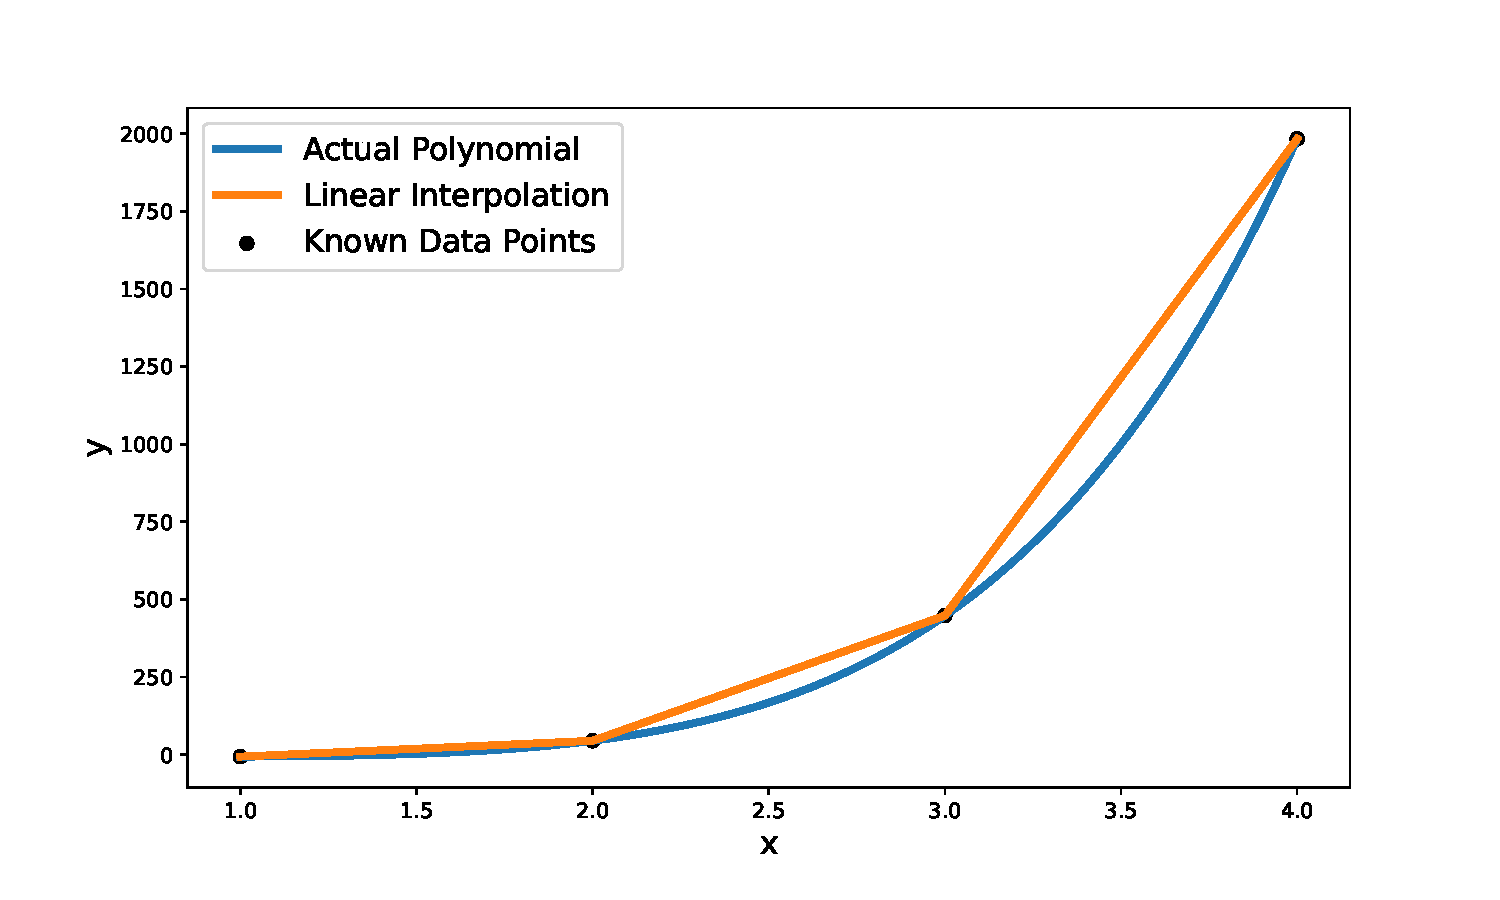
\includegraphics[height=0.6\textheight]{figs/linear_int}
\end{frame}
%
\begin{frame}{Linear interpolation}
\begin{itemize}
\item Linear interpolation in math
\begin{enumerate}
\item Assume $\underline{v}_{t+1}$ is known on grids $\mathcal{G}_{z}\times\mathcal{G}_{a}$
(tensor product)
\item Want to evaluate $\underline{v}_{t+1}(z^{i_{z}},a)$ for arbitrary
$a$ 
\item Find place in grid $\mathcal{G}_{a}$ where $a^{l}<a<a^{l+1}$ 
\item Compute interpolation:
\begin{align*}
\breve{\underline{v}}_{t+1}(z^{i_{z}},a) & =\underline{v}_{t+1}(z^{i_{z}},a^{l})+\omega(a-a^{l})\\
\omega & \equiv\frac{v_{t+1}(z^{i_{z}},a^{l+1})-v_{t+1}(z^{i_{z}},a^{l})}{a^{l+1}-a^{l}}\\
l & \equiv\text{largest }i_{a}\in\{0,1,\dots,\#_{a}-2\}\text{ such that }a^{i_{a}}\leq a
\end{align*}
\end{enumerate}
\end{itemize}
\end{frame}
%
\begin{frame}{Discretization of income process}
\begin{itemize}
\item <+-> Assume that idiosyncratic income $z_{t}$ follows an AR(1) process:
\[
\log z_{t}=\rho_{z}\log z_{t-1}+\psi_{t},\,\,\,\psi_{t}\sim\mathcal{N}(0,\sigma_{\psi}^{2})
\]
where $\mathcal{\mathbb{E}}[z_{t}]=1$
\item Since shocks $\psi_{t}$ are normally distributed $z_{t}$ is \textbf{continuous
$\Rightarrow$} Need to discretize 
\item <+->Tauchen (1986) or Rouwenhorst (1995): Can approximate AR(1) with
discrete \textbf{Markov chain} that features:
\begin{itemize}
\item Same variance 
\item Same serial correlation 
\end{itemize}
\item <+-> Use algorithm from either paper to get grid\textbf{ }$\mathcal{G}_{z}$
and transition probabilities $\left\{ \pi_{j,i}\right\} $ given $\rho_{z}$
and $\sigma_{\psi}$
\item <+-> Households move between states (points in $\mathcal{G}_{z}$)
with transition probability $\pi_{j,i}=\text{Pr}[z_{t}=z^{i}\,|\,z_{t-1}=z^{j}]$
\end{itemize}
\end{frame}
%
\begin{frame}{Transition probability matrix}

\centering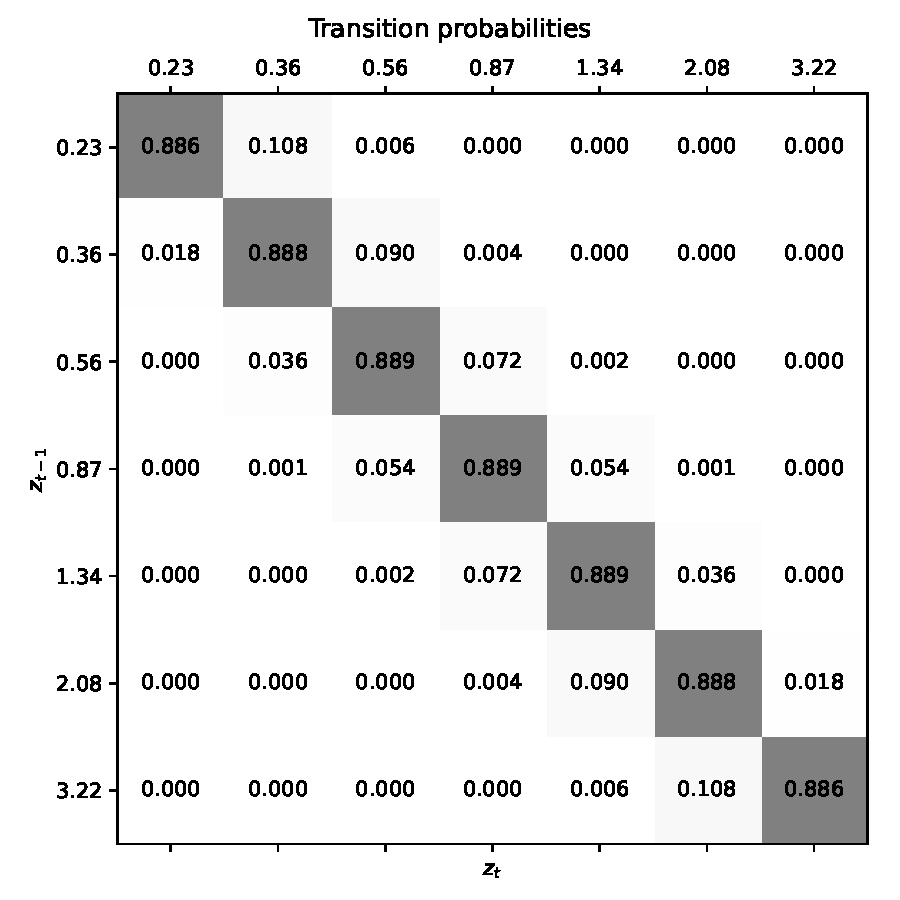
\includegraphics[height=0.8\textheight]{figs/z_trans}
\end{frame}
%
\begin{frame}{Value function iteration (VFI)}
\begin{itemize}
\item <+->\textbf{Beginning-of-period value function:
\[
\underline{v}_{t}(z^{i_{z-}},a^{i_{a-}})=\sum_{i_{z}=0}^{\#_{z}-1}\pi_{i_{z-},i_{z}}v_{t}(z^{i_{z}},a^{i_{a-}})
\]
}
\item <+->\textbf{End-of-period value-of-choice:}
\begin{align*}
v_{t}(z^{i_{z}},a^{i_{a-}}) & =\max_{c_{t}}v_{t}^{Choice}(z^{i_{z}},a^{i_{a-}}|c_{t})\\
 & \text{with }c_{t}\in[0,(1+r)a^{i_{a-}}+wz^{i_{z}}+\underline{a}]
\end{align*}
\vspace{-7mm}
\begin{align*}
v_{t}^{Choice}(z^{i_{z}},a^{i_{a-}}|c_{t}) & =u(c_{t})+\underline{\breve{v}}_{t+1}(z^{i_{z}},a_{t})\\
 & \text{with }a_{t}=(1+r)a^{i_{a-}}+wz^{i_{z}}-c_{t}
\end{align*}
\item <+->\textbf{Inner loop: }For each grid point in $\mathcal{G}_{z}\times\mathcal{G}_{a}$
find $c_{t}^{\ast}(z_{t},a_{t-1})$ and therefore $v_{t}(z_{t},a_{t-1})$
with a \emph{numerical optimizer}
\item <+->\textbf{Outer loop: }Backwards from $t=T-1$ (note $\underline{v}_{T}=0$,
or known)
\end{itemize}
\end{frame}
%
\begin{frame}{Convergence $(t=T-1-k)$}

\centering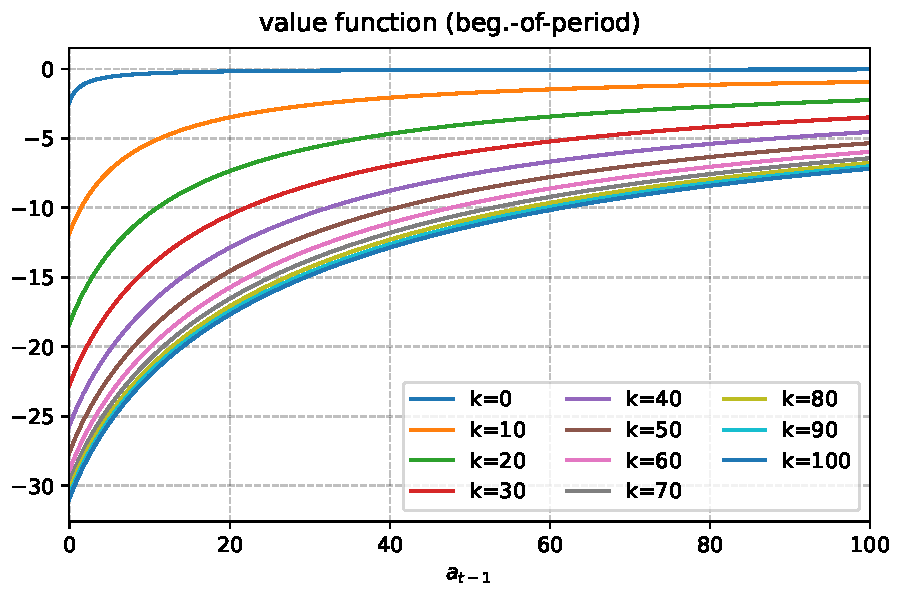
\includegraphics[width=0.5\textwidth]{figs/vbeg_func_convergence}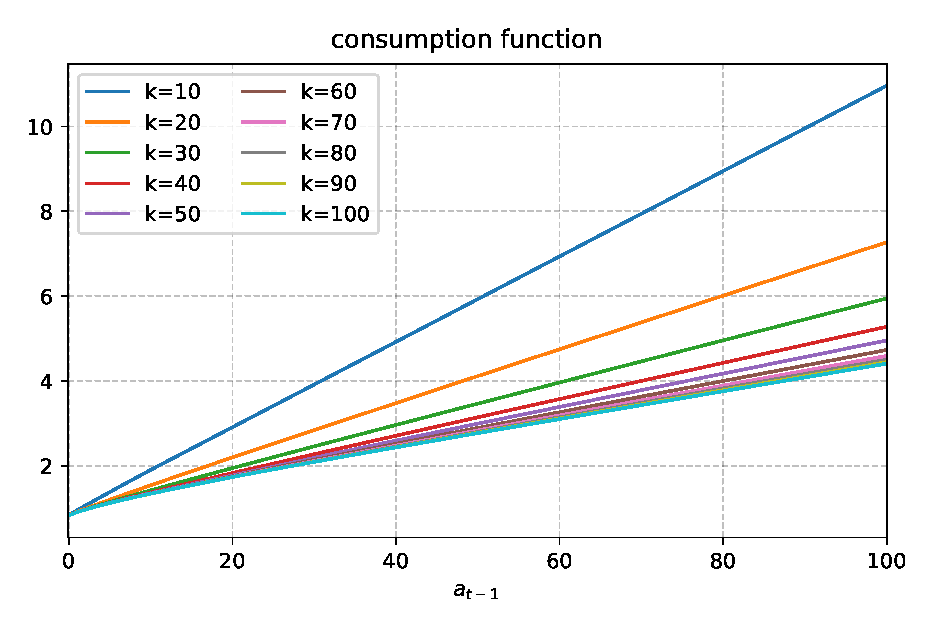
\includegraphics[width=0.5\textwidth]{figs/c_func_convergence}

with $z_{t}=0.87$
\end{frame}
%
\begin{frame}{Converged policy functions}

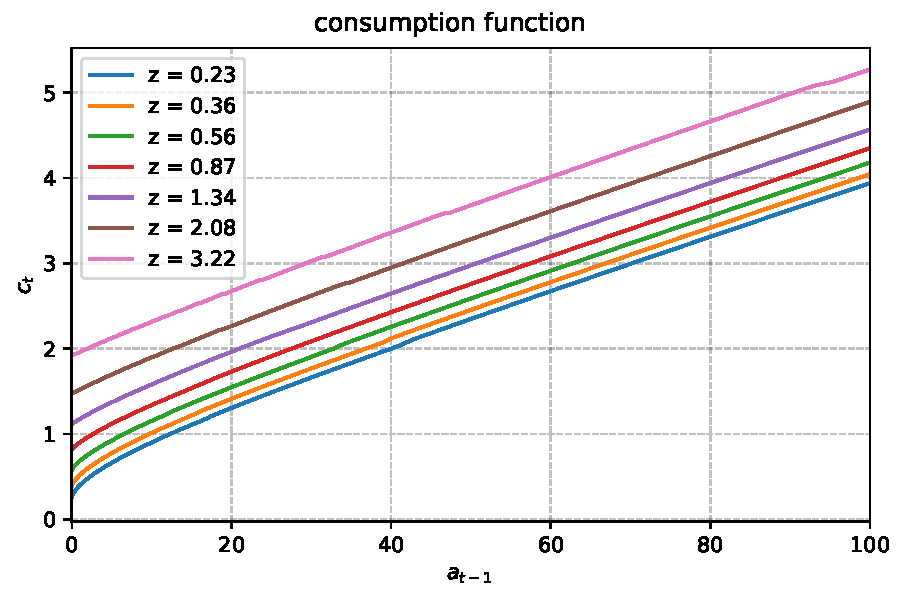
\includegraphics[width=0.5\textwidth]{figs/c_func}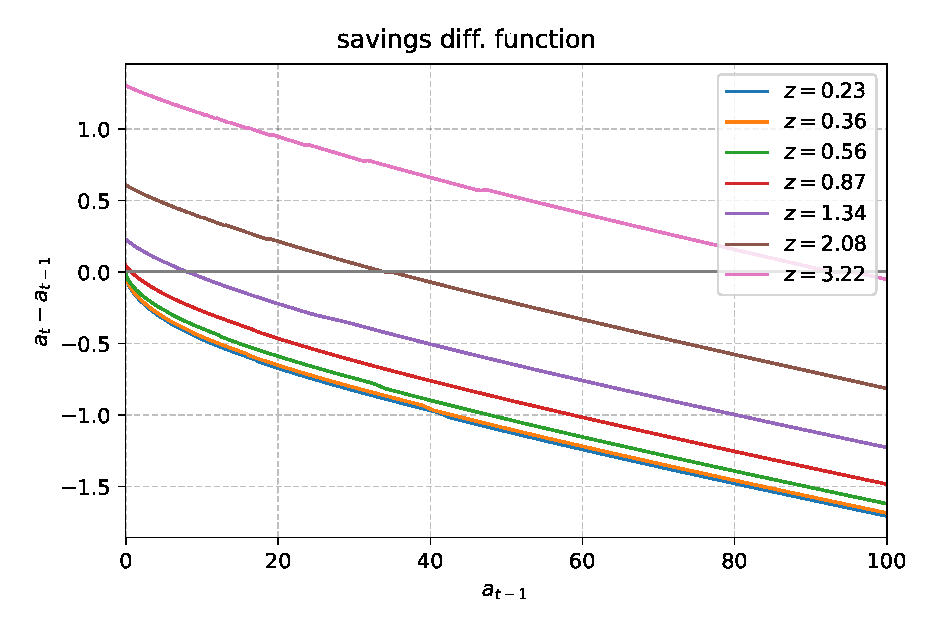
\includegraphics[width=0.5\textwidth]{figs/a_diff_func}

\textbf{Precautionary saving:}
\begin{itemize}
\item Consumption function \emph{concave} 
\item Savings drift imply buffer-stock target 
\begin{itemize}
\item Impatience vs. precautionary saving 
\end{itemize}
\end{itemize}
\end{frame}
%
\begin{frame}{Numerical Monte Carlo simulation}
\begin{itemize}
\item <+->\textbf{Initial distribution: }Draw $z_{i,-1}$ and $a_{i,-1}$
for $i\in\{0,1,\dots,N-1\}$ 
\item <+->\textbf{Simulation: }Forwards in time from $t=0$ and in each
time period
\begin{enumerate}
\item Draw $z_{it}$ given transition probabilities
\item Use linear interpolation to evaluate\vspace{-1mm} 
\begin{align*}
c_{it} & =\breve{c}_{t}^{\ast}(z_{it},a_{it-1})\\
a_{it} & =(1+r)a_{it-1}+wz_{it}-c_{it}
\end{align*}
\end{enumerate}
\item <+->\textbf{Review:}
\begin{itemize}
\item \textbf{Pro:} Simple to implement
\item \textbf{Con:} Computationally costly and introduces randomness $\Rightarrow$
Need large $N$ to avoid noise 
\end{itemize}
\end{itemize}
\end{frame}
%
\begin{frame}{Numerical histogram simulation - general idea}
\begin{itemize}
\item Alternative to Monte Carlo simulation that avoids stochasticity: \textbf{histogram
method}
\item <+-> End goal: obtain discretized distribution directly on the grids
$\mathcal{G}_{z}\times\mathcal{G}_{a}$
\item <+-> If households only make choices on grid (i.e. no continuous
choice) then obtain distribution as follows:
\begin{itemize}
\item \textbf{Initial distribution: }Choose $\underline{\boldsymbol{D}}_{0}(z_{-1},a_{-1})$,
which is defined on $\mathcal{G}_{z}\times\mathcal{G}_{a}$ and sum
to $1$ $\equiv$ \emph{histogram}
\item \textbf{Simulation: }Forwards in time from $t=0$ and in each time
period
\begin{enumerate}
\item \textbf{Distribute stochastic mass:} For each $i_{z}$ and $i_{a-}$
calculate\vspace{1mm}

$\boldsymbol{D}_{t}(z^{i_{z}},a^{i_{a-}})=\sum_{i_{z-}=0}^{\text{\#}_{z}-1}\pi_{i_{z-},i_{z}}\boldsymbol{\underline{\boldsymbol{D}}}_{t}(z^{i_{z-}},a^{i_{a-}})$\vspace{1mm}
\item \textbf{Initial zero mass:} Set $\underline{\boldsymbol{D}}_{t+1}(z^{i_{z}},a^{i_{a}})=0$
for all $i_{z}$ and $i_{a}$
\item \textbf{Distribute endogenous mass:} For each $i_{z}$ and $i_{a-}$
do:
\item Find $l\equiv i_{a}\in\{0,1,\dots,\#_{a}-2\}$ such that $a_{t}^{\ast}(z^{i_{z}},a^{i_{a-}})=a^{l}$
(on grid assumption)
\item Increment $\underline{\boldsymbol{D}}_{t+1}(z^{i_{z}},a^{l})$ with
$\boldsymbol{D}_{t}(z^{i_{z}},a^{i_{a-}})$
\end{enumerate}
\end{itemize}
\end{itemize}
\end{frame}
%
\begin{frame}{Numerical histogram simulation I}
\begin{itemize}
\item If households may choose savings policy $a_{t}^{\ast}(z^{i_{z}},a^{i_{a}})$
which is not on the grid $\mathcal{G}_{a}$ how do we distribute mass
across the grid?
\item <+-> Use >>lottery<<: Find neighbouring grid points for policy
function $a^{l}<a_{t}^{\ast}(z^{i_{z}},a^{i_{a}})<a^{l+1}$
\item <+-> Assume that a fraction $\omega$ of households goes to $a^{l}$,
remaining share goes to $a^{l+1}$
\item <+-> Weight $\omega$ should satisfy:
\[
\omega a^{l}+\left(1-\omega\right)a^{l+1}=a_{t}^{\ast}(z^{i_{z}},a^{i_{a}})
\]
Such that we get right asset level on average. 
\item <+->Solve for weight:
\[
\omega=\frac{a^{l+1}-a^{\ast}(z^{i_{z}},a^{i_{a}})}{a^{l+1}-a^{l}}
\]
\end{itemize}
\end{frame}
%
\begin{frame}{Numerical histogram simulation II}
\begin{itemize}
\item <+->\textbf{Initial distribution: }Choose $\underline{\boldsymbol{D}}_{0}(z_{-1},a_{-1})$,
which is defined on $\mathcal{G}_{z}\times\mathcal{G}_{a}$ and sum
to $1$ $\equiv$ \emph{histogram}
\item <+->\textbf{Simulation: }Forwards in time from $t=0$ and in each
time period
\begin{enumerate}
\item <+->\textbf{Distribute stochastic mass:} For each $i_{z}$ and $i_{a-}$
calculate\vspace{1mm}

$\boldsymbol{D}_{t}(z^{i_{z}},a^{i_{a-}})=\sum_{i_{z-}=0}^{\text{\#}_{z}-1}\pi_{i_{z-},i_{z}}\boldsymbol{\underline{\boldsymbol{D}}}_{t}(z^{i_{z-}},a^{i_{a-}})$\vspace{1mm}
\item <+->\textbf{Initial zero mass:} Set $\underline{\boldsymbol{D}}_{t+1}(z^{i_{z}},a^{i_{a}})=0$
for all $i_{z}$ and $i_{a}$\vspace{2mm}
\item <+->\textbf{Distribute endogenous mass:} For each $i_{z}$ and $i_{a-}$
do\vspace{1mm}
\begin{enumerate}
\item <+->Find $l\equiv\text{largest }i_{a}\in\{0,1,\dots,\#_{a}-2\}$
such that $a^{i_{a}}\leq a_{t}^{\ast}(z^{i_{z}},a^{i_{a-}})$\vspace{1mm}
\item <+->Calculate $\omega=\frac{a^{l+1}-a^{\ast}(z^{i_{z}},a^{i_{a-}})}{a^{l+1}-a^{l}}\in[0,1]$\vspace{1mm}
\item <+->Increment $\underline{\boldsymbol{D}}_{t+1}(z^{i_{z}},a^{l})$
with $\omega\boldsymbol{D}_{t}(z^{i_{z}},a^{i_{a-}})$\vspace{1mm}
\item <+->Increment $\boldsymbol{\underline{\boldsymbol{D}}}_{t+1}(z^{i_{z}},a^{l+1})$
with $(1-\omega)\boldsymbol{D}_{t}(z^{i_{z}},a^{i_{a-}})$\vspace{-1mm}
\end{enumerate}
\end{enumerate}
\item <+->\textbf{Review:}
\begin{enumerate}
\item \textbf{Pro: }Computationally efficient and no randomness
\item \textbf{Con: }Introduces a non-continuous distribution
\end{enumerate}
\end{itemize}
\end{frame}
%
\begin{frame}{Small example}
\begin{itemize}
\item \textbf{Grids:} $\mathcal{G}_{z}=\{\underline{z},\overline{z}\}$
and $\mathcal{G}_{a}=\{0,1\}$
\item \textbf{Transition matrix:} $\pi_{0,0}=\pi_{1,1}=0.5$
\item \textbf{Policy function: }
\begin{itemize}
\item Low income: $a^{\ast}(\underline{z},0)=a^{\ast}(\underline{z},1)=0$
\item High income: Let $a^{\ast}(\overline{z},0)=0.5$ and $a^{\ast}(\overline{z},1)=1$
\end{itemize}
\item \textbf{Initial distribution}: $\underline{\boldsymbol{D}}_{0}(z_{it},a_{it-1})=\begin{cases}
1 & \text{if }z_{it}=\underline{z}\text{ and }a_{it}=0\\
0 & \text{else}
\end{cases}$
\item \textbf{Task: }Calculate by hand the transitions to
\[
\boldsymbol{D}_{0},\,\underline{\boldsymbol{D}}_{1},\,\boldsymbol{D}_{1},\dots
\]

\emph{See simple simple\_histogram\_simulation.xlsx}
\end{itemize}
\end{frame}
%
\begin{frame}{Infinite horizon: $T\rightarrow\infty?$}
\begin{itemize}
\item \textbf{Initial guess: }Can be arbitrary. 
\begin{enumerate}
\item Everyone in one grid point, or
\item Ergodic distribution of $z_{it}$ and everyone has zero savings,
\end{enumerate}
\item \textbf{Convergence:} Simulate forward until the distribution does
not change anymore (given some tolerance)
\end{itemize}
\end{frame}
%
\begin{frame}{Converged CDF of savings}

\centering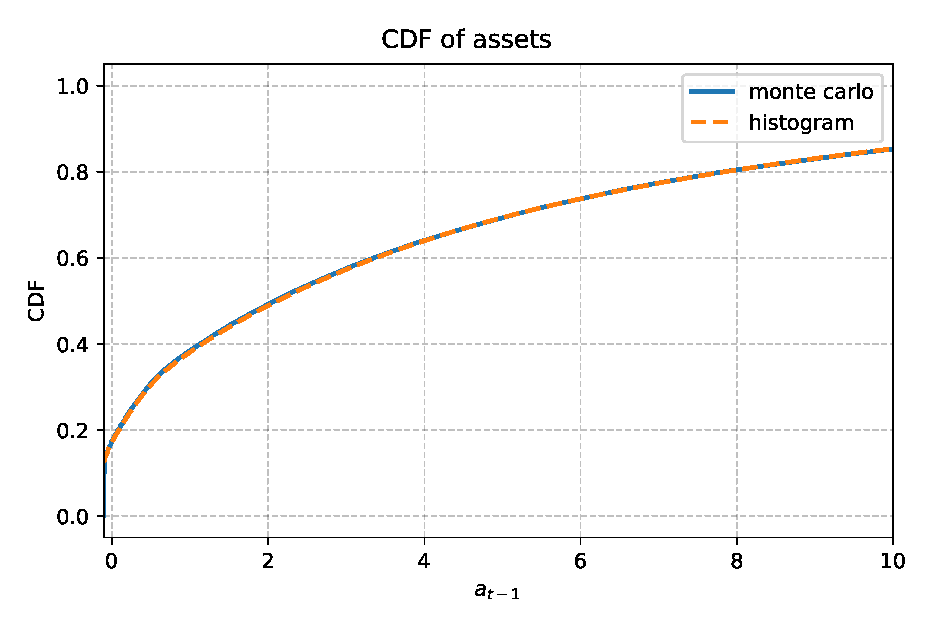
\includegraphics[height=0.8\textheight]{figs/a_cdf}
\end{frame}
%
\begin{frame}{MPCs}

\centering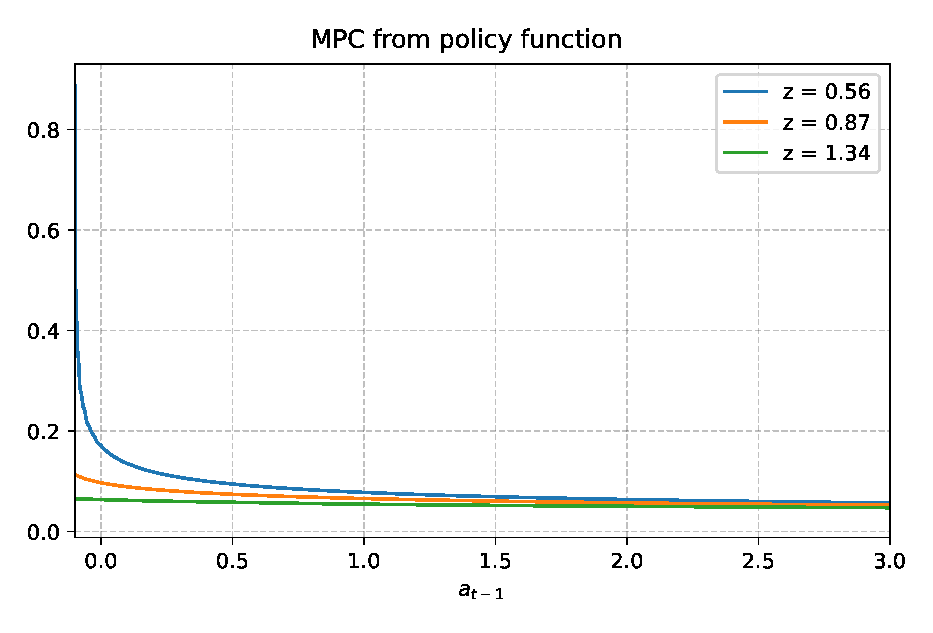
\includegraphics[width=0.5\textwidth]{figs/MPC_policy}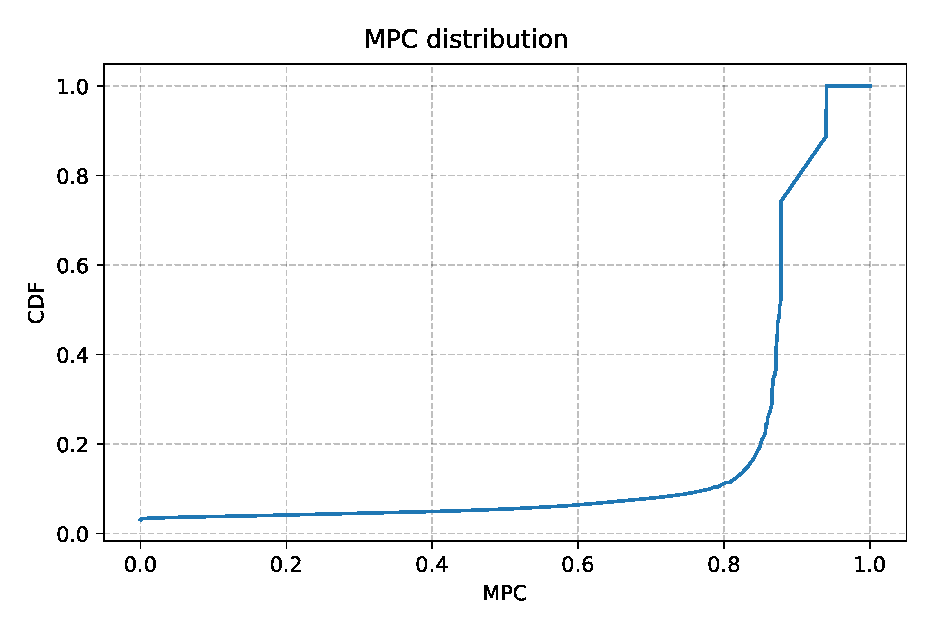
\includegraphics[width=0.5\textwidth]{figs/MPC_dist}
\end{frame}
%
\begin{frame}{Side-note: Matrix formulation}
\begin{itemize}
\item The histogram method can be written in \textbf{matrix form}:
\begin{align*}
\boldsymbol{D}_{t} & =\Pi_{z}^{\prime}\underline{\boldsymbol{D}}_{t}\\
\underline{\boldsymbol{D}}_{t+1} & =\Lambda_{t}^{\prime}\boldsymbol{D}_{t}
\end{align*}
\vspace{-2mm}where\vspace{3mm}
\begin{itemize}
\item []$\underline{\boldsymbol{D}}_{t}$ is vector of length $\#_{z}\times\#_{a}$
\vspace{2mm}
\item []$\boldsymbol{D}_{t}$ is vector of length $\#_{z}\times\#_{a}$
\vspace{2mm}
\item []$\Pi_{z}^{\prime}$ is derived from the $\pi_{i_{z-},i_{z}}$'s\vspace{2mm}
\item []\textbf{$\Lambda_{t}^{\prime}$ }is derived from the $l$'s and
$\omega$'s
\end{itemize}
\item \textbf{Note:} Example shown in notebook
\item \textbf{Further details: }Young (2010), Tan (2020),\\
Ocampo and Robinson (2022)
\end{itemize}
\end{frame}
%

\section{EGM}
\begin{frame}{Characteristics of VFI}
\begin{itemize}
\item <+->Value function iteration (VFI) is the standard method for solving
dynamic programs 
\begin{itemize}
\item Robust 
\item Easy to implement for a wide class of models 
\item Well known convergence properties (c.f. contraction mapping theorem)
\end{itemize}
\item <+->But significant drawbacks in terms of \textbf{computational speed}
\begin{itemize}
\item Computationally expensive since we have to use a numerical optimizer
at every point in the state space 
\item Have to do interpolation at every evaluation of the optimization problem 
\end{itemize}
\item <+->Solution: \textbf{Endogenous grid-point method} 
\end{itemize}
\end{frame}
%
\begin{frame}{Endogenous grid-point method (EGM)}

Alternative to VFI using Euler, i.e. $c_{t}^{-\sigma}=\beta(1+r)\mathbb{E}_{t}[c_{t+1}^{-\sigma}]$:
\begin{enumerate}
\item <+->Calculate\textbf{ post-decision marginal value of cash:}\vspace{-1mm}
\[
q(z^{i_{z}},a^{i_{a}})=\sum_{i_{z+}=0}^{\#_{z}-1}\pi_{i_{z},i_{z+}}c_{+}(z^{i_{z+}},a^{i_{a}})^{-\sigma}
\]
\item <+->\vspace{-2mm}\textbf{Invert Euler-equation:}\vspace{-1mm}
\[
c(z^{i_{z}},a^{i_{a}})=(\beta(1+r)q(z^{i_{z}},a^{i_{a}}))^{-\frac{1}{\sigma}}
\]
\item <+->\vspace{-1mm}\textbf{Endogenous cash-on-hand:}\vspace{-1mm}
\[
m(z^{i_{z}},a^{i_{a}})=a^{i_{a}}+c(z^{i_{z}},a^{i_{a}})
\]
\item <+->\vspace{-1mm}\textbf{Consumption function:} Calculate $m=(1+r)a^{i_{a-}}+wz^{i_{z}}$

If $m\leq m(z^{i_{z}},a^{0})$ constraint binds: $c^{\ast}(z^{i_{z}},a^{i_{a-}})=m+\underline{a}$

Else: $c^{\ast}(z^{i_{z}},a^{i_{a-}})=$ interpolate $m(z^{i_{z}},:)$
to $c(z^{i_{z}},:)$ at $m$
\end{enumerate}
\end{frame}
%

\section{Practice}
\begin{frame}{In practice}
\begin{itemize}
\item \textbf{EconModel: }Go through notebook {\color{DarkRed}\href{https://github.com/NumEconCopenhagen/EconModelNotebooks}{01. Using the EconModelClass}}
(except part on C++)
\item \textbf{ConSav: }Look at the {\color{DarkRed}\href{https://github.com/NumEconCopenhagen/ConsumptionSavingNotebooks}{04. Tools}}
folder.
\item \textbf{Todays notebook: }\emph{Consumption-Saving Model} show implementation
of solution and simulation methods.
\end{itemize}
\end{frame}
%

\section{Summary}
\begin{frame}{Summary and next week}
\begin{itemize}
\item \textbf{Today: }
\begin{enumerate}
\item Introduction to course
\item Consumption-saving models
\item Numerical dynamic programming
\end{enumerate}
\item \textbf{Next week: }More on consumption-saving models
\item \textbf{Homework:}
\begin{enumerate}
\item Ensure that your Python installation is working, and that you can
use ConSav, GEModelTools
\item Familiarize your self with today's code and the basic concepts of
dynamic programming 
\end{enumerate}
\end{itemize}
\end{frame}
%

\end{document}
